\section{Semantische Analyse}

\begin{frame}
\frametitle{Semantische Analyse}

\begin{enumerate}
\item Auflösung von Importen
\item Modulnormalisierung
\item Datentypen und Funktionen überprüfen
\item Type-Checking
\end{enumerate}

\end{frame}


\begin{frame}[containsverbatim=true]
\frametitle{Import-Überprüfung}

\begin{itemize}
\item Import-Anweisung: Paar aus Pfad und Bezeichner
	\begin{verbatim}
	IMPORT "path/to/module" AS MyModule
	\end{verbatim}
\item eineindeutige Modul-Bezeichner-Zuordnung
\item Annahme: genau ein Pfad identifiziert ein Modul
\item erlaubte Pfade:
	\begin{itemize}
	\item Kleinbuchstaben
	\item Zahlen
	\item Minus (-) und Unterstrich (\_)
	\item relative Pfade
	\end{itemize}
\end{itemize}

\end{frame}


\begin{frame}[containsverbatim=true]
\frametitle{Modulnormalisierung}

\begin{itemize}
\item keine modulübergreifende Modul-Bezeichner-Zuordnung
\item Normalisierung erforderlich
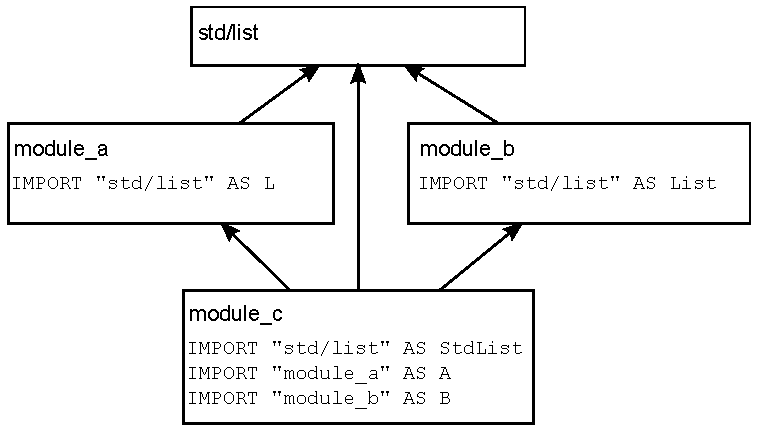
\includegraphics[width=1\linewidth]{depsModABC}
\item Substitution von \verb+L+ bzw. \verb+List+ durch \verb+StdList+
\end{itemize}


\end{frame}


\begin{frame}
\frametitle{Kontextprüfung}

\begin{itemize}
\item Berücksichtigung von importierten Datentypen und Funktionen
\item initialer Kontext um Modulkontext erweitert
\item Type-Checker weitestgehend unverändert
\end{itemize}

\end{frame}
